% ************ Capítulo 1 ************
%\renewcommand{\chaptername}{Capítulo}
\chapter{Introdução}
\label{cap:1}

\section{Enquadramento}
Em Portugal o uso de vela de cera é uma pratica bastante decorrente. Estas são usadas para iluminação, como elementos decorativos e para o culto ao mortos. Todos os anos milhares de velas são utilizadas em território nacional, nomeadamente círios. Os círios são particularmente frequentes em cemitérios. Constituídos por um envolucro em plástico e com uma tampa em metal são vistos como elemento obrigatório na homenagem a um ente querido falecido. Pela quantidade de velas que são queimadas diariamente os resíduos destas amontoam-se e a solução que é vista para este problema é o colocar o que resta do círio no caixote do lixo indiferenciado. Esta situação acarreta vários problemas ambientais que a médio prazo podem ter consequências mais gravosas, como por exemplo, infestação de vespas e abelhas uma vez que estes animais usam a cera das velas para construir as suas estruturas de abrigo.
A reciclagem de resíduos de velas ainda não é neste momento uma atividade com grande expressão no mercado Português. Existem apenas algumas empresas atualmente a fazer a reciclagem deste tipo de resíduos e as suas principais fontes de materia-prima são os cemitérios e locais de culto religioso, onde o uso de velas é uma pratica muito comum. Entre as entidades que operam neste setor podemos mencionar o Santuário de Fátima\cite{Destak2010}, o Centro Ambiental do Carvalho de Calvos\cite{SecundinoCunha2016} e a Natural Life\cite{NaturalLife}.

\section{Apresentação da empresa}
A Natural Life, Lda. é uma empresa fundada em 2013. Está sediada na rua de Terramonte nº 781, Armazém C20, na Maia. Tendo como atividade a recolha e reciclagem de resíduos de velas, a Natural Life surge como uma empresa ecológica, inteiramente ligada a área ambiental, mais concretamente à reciclagem\cite{NaturalLife}. A empresa cuida de todo o processo, desde a recolha da materia-prima nos cemitérios com as quais tem parceria, a separação do corpo de plastico, da tampa de metal e da cera até à fundição da cera. Em alguns casos a recolha do material é substituída por material recolhido por terceiros, mantendo-se o resto do processo. A fábrica está dividida em duas áreas especificas: a zona de armazém, cargas e descargas e a zona de processamento dos círios, conforme descrito na plata da figura \ref{fig:planta_naturallife}. Os registos da fábrica são feitos numa base de dados muito simples, com vários tipos de limitações que inibem a empresa de poder expandir.

\section{Objetivos}
Implementar um sistema de informação (SI\label{sym:SI}) para efetuar o registo do ponto dos colaboradores, recolhas, produção, acabamento e saída do produto. Esta solução teria de possuir duas áreas distintas, a primeira destinada ao uso na fábrica e a segunda destinada ao uso pela administração. Pretende-se ainda que esta seja uma solução bem integrada no processo da empresa e que traga o leve tempo possível de adaptação ao novo sistema por parte dos funcionários.

\section{Calendarização}
Para descrever a calendarização da Unidade Curricular (UC\label{sym:UC}) PROjeto/EStágio (PROES\label{sym:PROES}) da Licenciatura em Engenharia de Sistemas (LES).

\begin{figure}[htbp] 
	\begin{center}
		% Requires \usepackage{graphicx}
		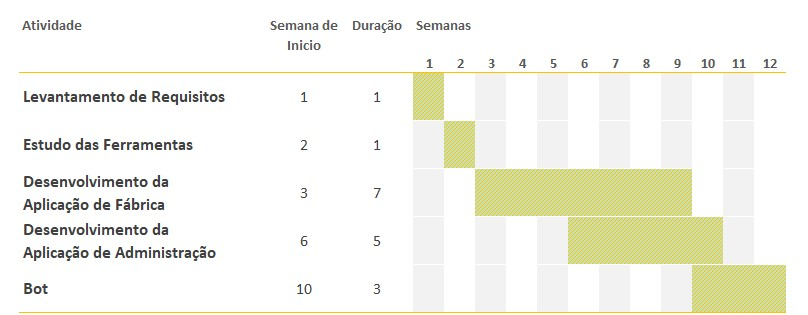
\includegraphics[width=\textwidth,keepaspectratio]{figuras/DiagramaGant.jpg}
		\caption{Planemento - diagrama de Gantt}
		\label{fig:gantt chart} 
	\end{center}
\end{figure}

\section{Organização do relatório}
No Capítulo 1 é feito o enquadramento do projeto dando uma visão alto nível do projeto. No capítulo 2, é apresentado o estado da arte. É neste capitulo que são descritas as diferentes opções para a realização do projeto e onde são descritas as escolhas feitas e o seu motivo. No capítulo 3 é apresentada a lista de requisitos e do projeto, bem como o processo para a sua obtenção. O capítulo 4, destina-se à projeção do sistema descrevendo o modo como os elementos do sistema se interligam entre si, para no capítulo 5 ser descrito o processo de implementação e a sua execução. No último capítulo, o 6º, são apresentadas as conclusões do projeto e os resultados da mesmo, analisando o \textit{feedback} geral recebido pela administração e pelos colaboradores da empresa. É ainda neste capitulo que é feita a analise critica do estudante face ao trabalho desenvolvido.
